
\includegraphics[height=1.25cm]{images/pictograms/replication}

\includegraphics[height=1.25cm]{images/pictograms/benchmark}

\includegraphics[height=1.25cm]{images/pictograms/triangle}

\includegraphics[height=1.25cm]{images/pictograms/under_construction}

\includegraphics[height=1.25cm]{images/pictograms/FEM}

\includegraphics[height=1.25cm]{images/pictograms/paraview}

%%%%%%%%%%%%%%%%%%%%%%%%%%%%%%%%%%%%%%%%%%%%%%%%%%%%%%%%%%%%%%%%%%%%%%%%%%%%%%%%%%%%%%%%%%%%%%%%%%%


\lstinputlisting[language=bash,basicstyle=\small]{python_codes/fieldstone_62/keywords.ascii}

\begin{center}
Code at \url{https://github.com/cedrict/fieldstone/tree/master/python_codes/fieldstone_62}
\end{center}

\par\noindent\rule{\textwidth}{0.4pt}

\index{stopics}{$P_2^+\times P_{-1}$}
%%%%%%%%%%%%%%%%%%%%%%%%%%%%%%%%%%%%%%%%%%%%%%%%%%%%%%%%%%%%%%%%%%%%%%%%%%%%%%%%%%%%%%%%%%%%

The setup is presented in the phd thesis (chapter 4) of M. Quinquis \cite{quin14},
In this stone we focus on the case 1 of his work and only solve the system once (single time step).
The domain is $1500\times 670$ km. 

The setup and the boundary conditions are shown hereunder:
\begin{center}
\includegraphics[width=\linewidth]{python_codes/fieldstone_62/images/quin14_setup}\\
{\captionfont Model setup for subduction of a 70 Ma old oceanic plate under a 40 Ma
old oceanic plate. A) Setup of the whole model. The top, bottom, and left boundaries
are free-slip, while the right boundary condition includes material in- and outflow. S HB :
Serpentinised Harzburgite, and B OC : Bulk Oceanic Composition. The ‘thermal’ layers
are only required in the linear viscous models. B) Zoom of the setup at the trench, h is the
thickness of the weak zone. C) Definition of the in- and outflow velocities on the right
boundary. Taken from \cite{quin14}}
\end{center}

As opposed to the original benchmarking effort carried out by Quinquis and collaborators
I build the mesh with triangles so that I can exactly represent the layers (and especially 
the weak zone) with an adequate resolution. The elements used are the Crouzeix-Raviart one
(see Section~\ref{MMM-sec:crouzeix-raviart}). 

In {points.py} the coordinates of the key points are defined. The {generate\_nodes.py}
script generates the input file for 
the {\sl triangle} program\footnote{\url{https://www.cs.cmu.edu/~quake/triangle.html}}. 
Finally the {fieldstone.py} script 
reads in the mesh, sets up the material layout, the boundary conditions and solves the 
FE system. Simply use the {\sl run} script to trigger the mesh generation and the FE 
calculations.  
Note that the compiled {\sl triangle} executable file (as compiled by you 
on your own machine) must be present in this folder.

\begin{center}
\includegraphics[width=\linewidth]{python_codes/fieldstone_62/results/mats1}\\
{\captionfont Taken from \cite{quin14}}
\end{center}

The letters referenced in the {points.py} file are shown hereunder:

\begin{center}
\includegraphics[width=11cm]{python_codes/fieldstone_62/images/setup1}\\
\includegraphics[width=11cm]{python_codes/fieldstone_62/images/setup2}
\end{center}


In this case 1, all materials are characterised by a constant density and a Newtonian rheology:
\begin{center}
\includegraphics[width=5cm]{python_codes/fieldstone_62/images/quin14_mats}
\end{center}

\newpage
\begin{center}
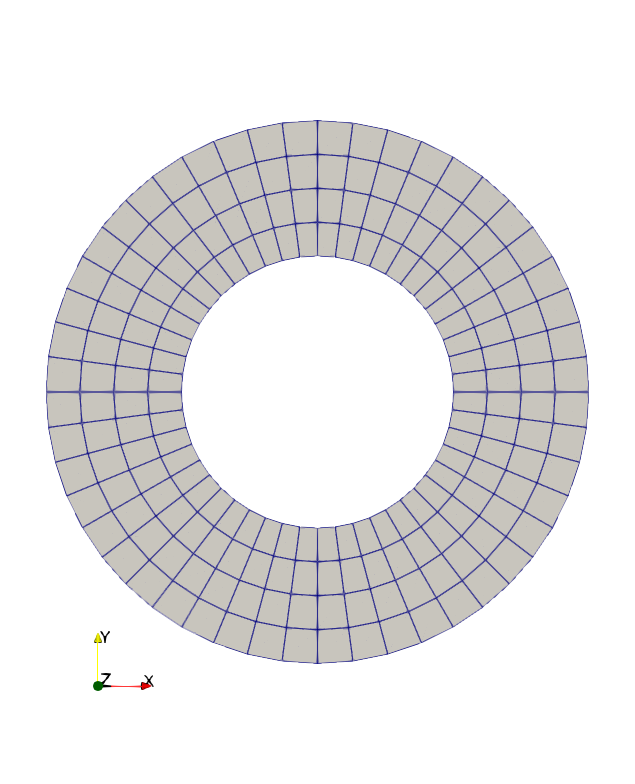
\includegraphics[width=13cm]{python_codes/fieldstone_62/results/mesh1}\\
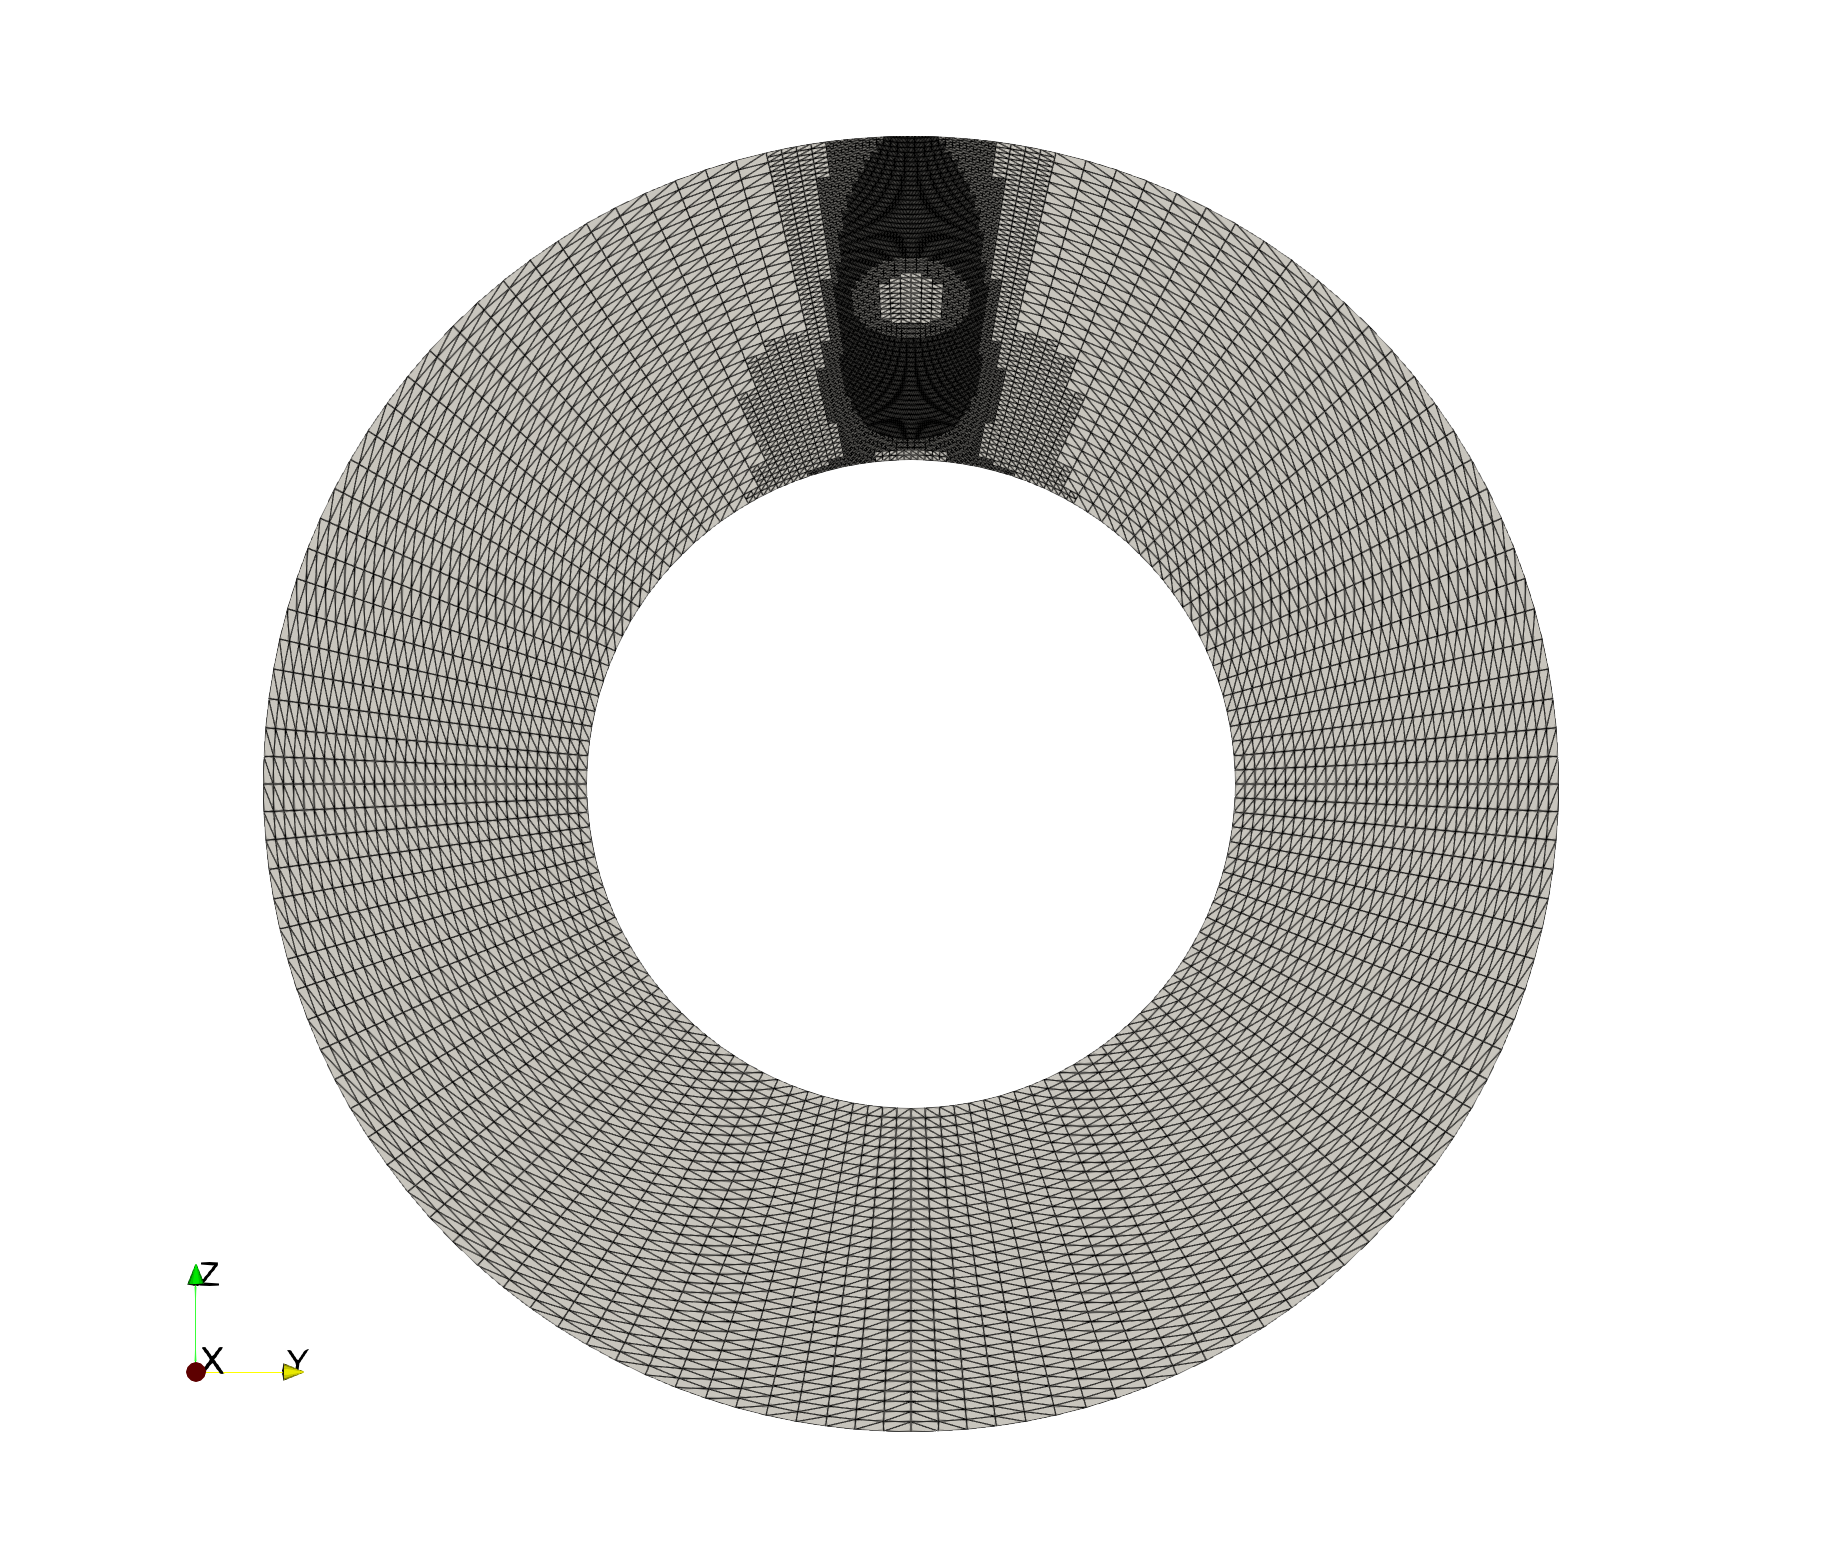
\includegraphics[width=13cm]{python_codes/fieldstone_62/results/mesh2}\\
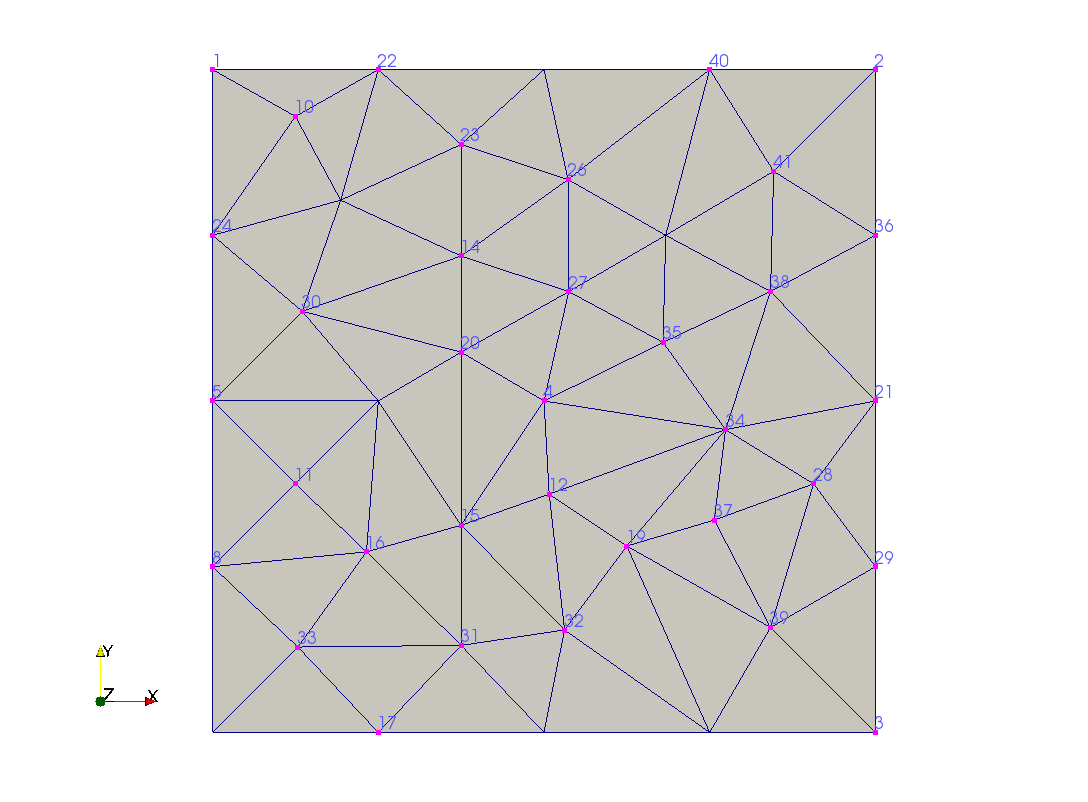
\includegraphics[width=13cm]{python_codes/fieldstone_62/results/mesh3}
\end{center}

\newpage
\begin{center}
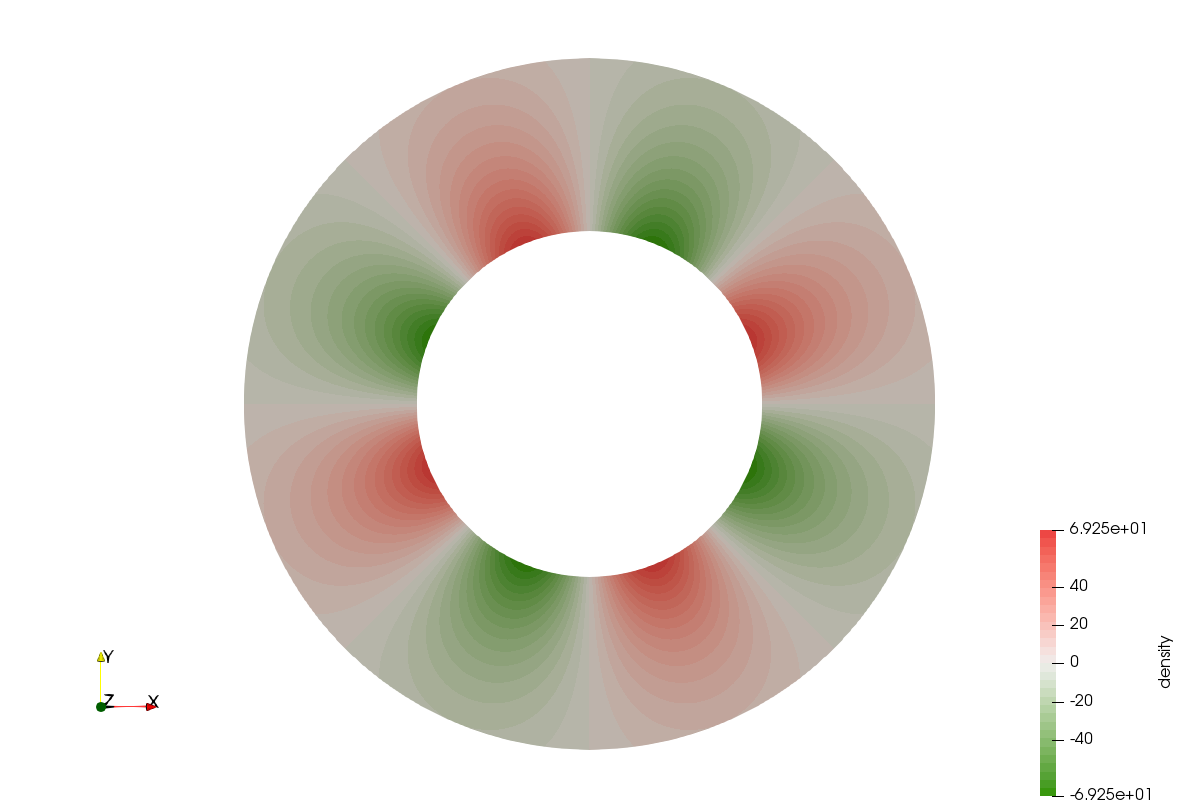
\includegraphics[width=12.5cm]{python_codes/fieldstone_62/results/density}\\
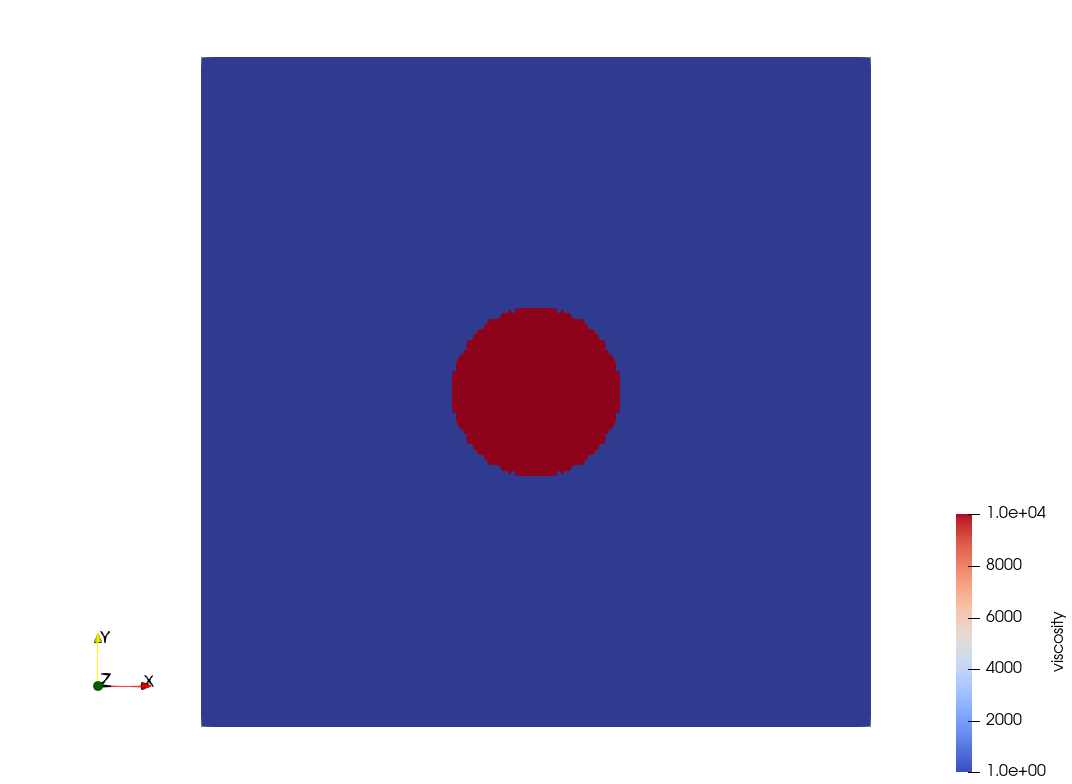
\includegraphics[width=12.5cm]{python_codes/fieldstone_62/results/viscosity}\\
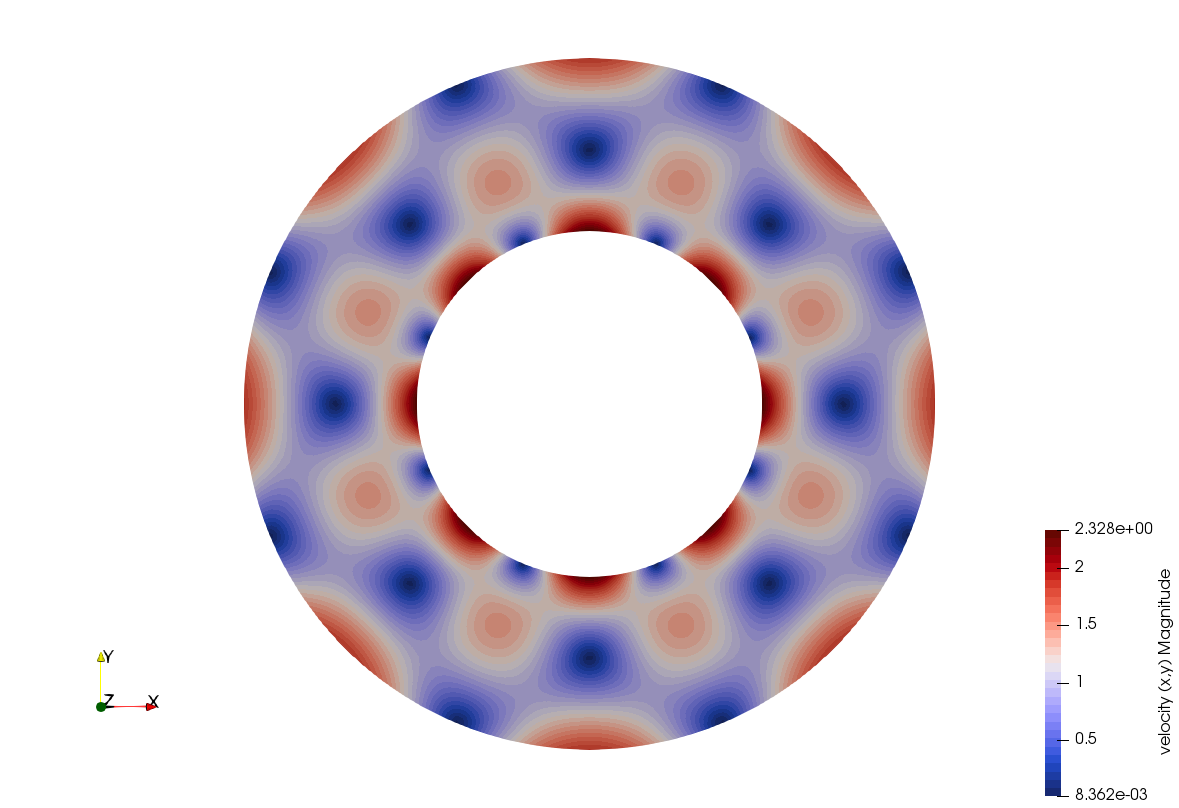
\includegraphics[width=12.5cm]{python_codes/fieldstone_62/results/velocity}\\
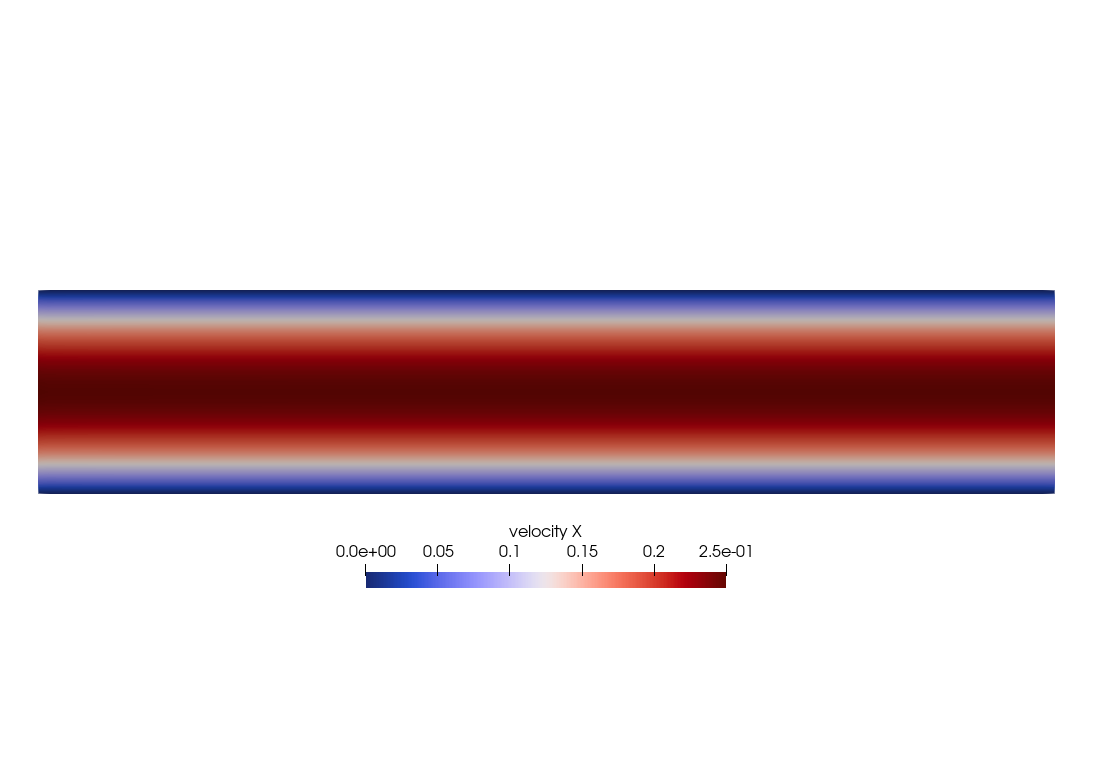
\includegraphics[width=12.5cm]{python_codes/fieldstone_62/results/u}\\
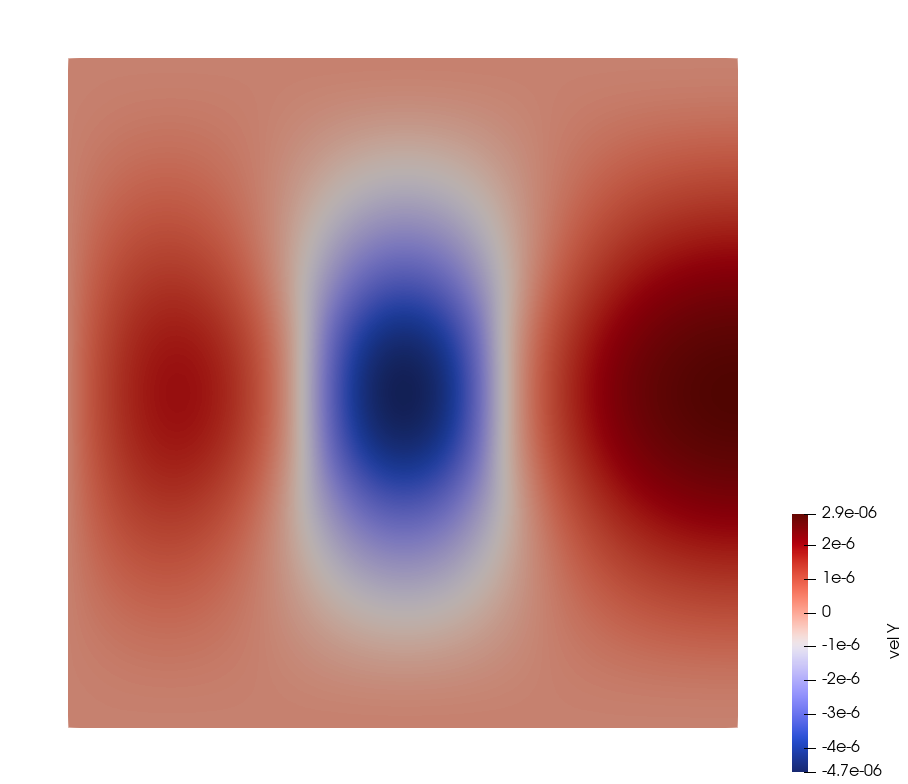
\includegraphics[width=12.5cm]{python_codes/fieldstone_62/results/v}\\
\end{center}

\newpage
\begin{center}
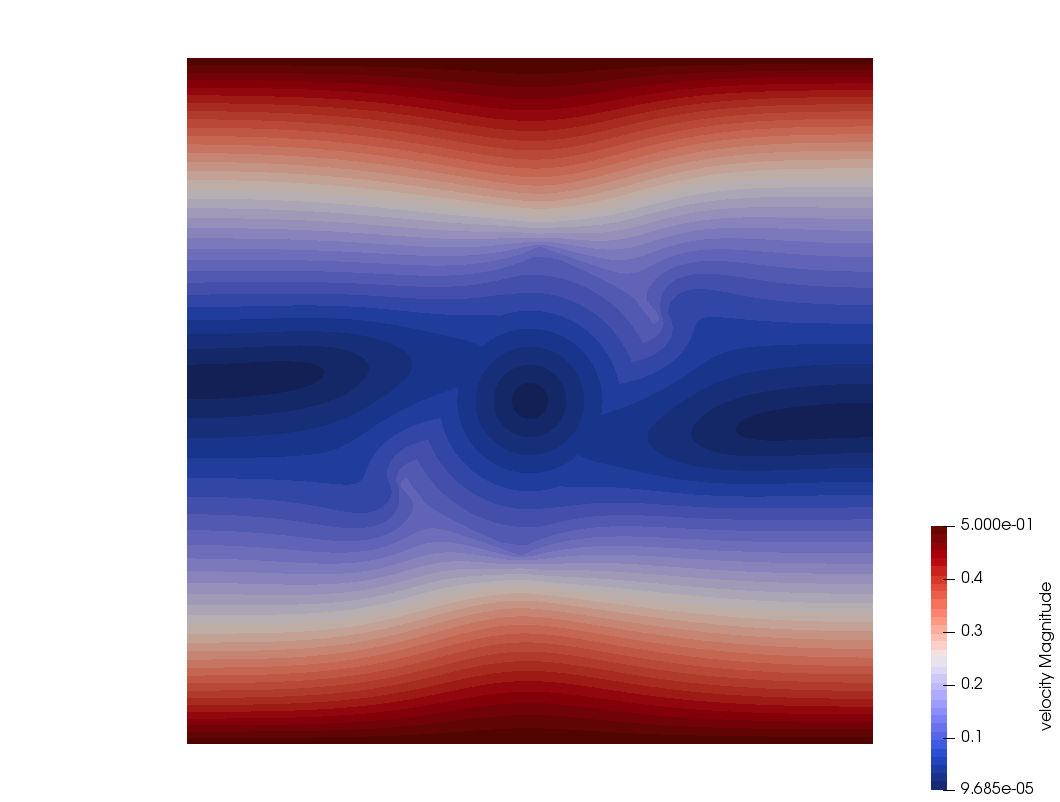
\includegraphics[width=10cm]{python_codes/fieldstone_62/results/vel2}\\
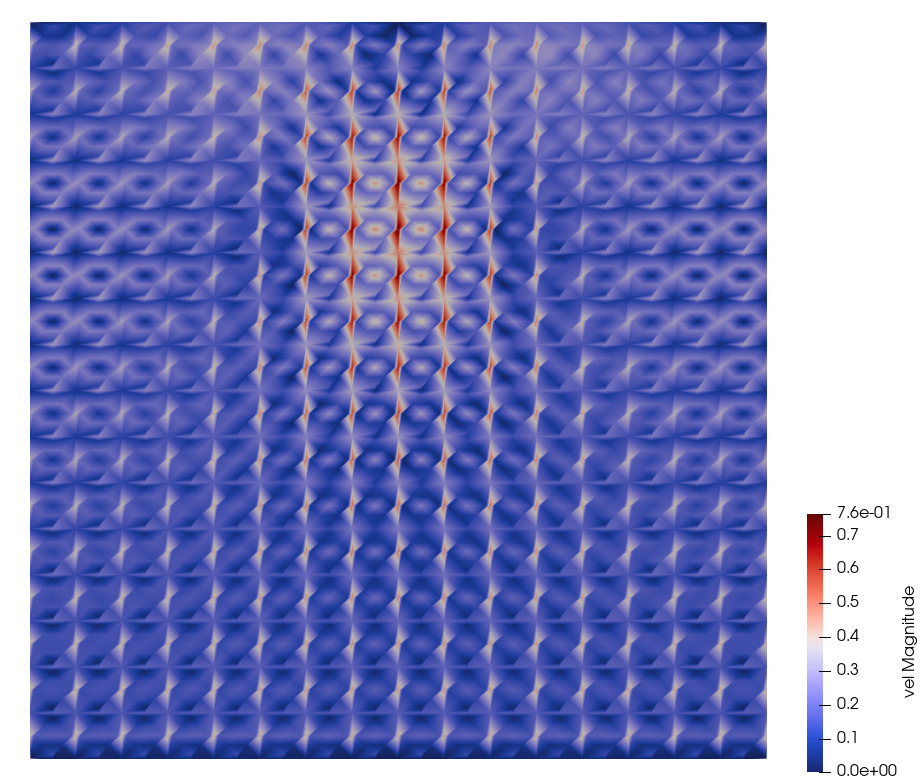
\includegraphics[width=10cm]{python_codes/fieldstone_62/results/vel3}\\
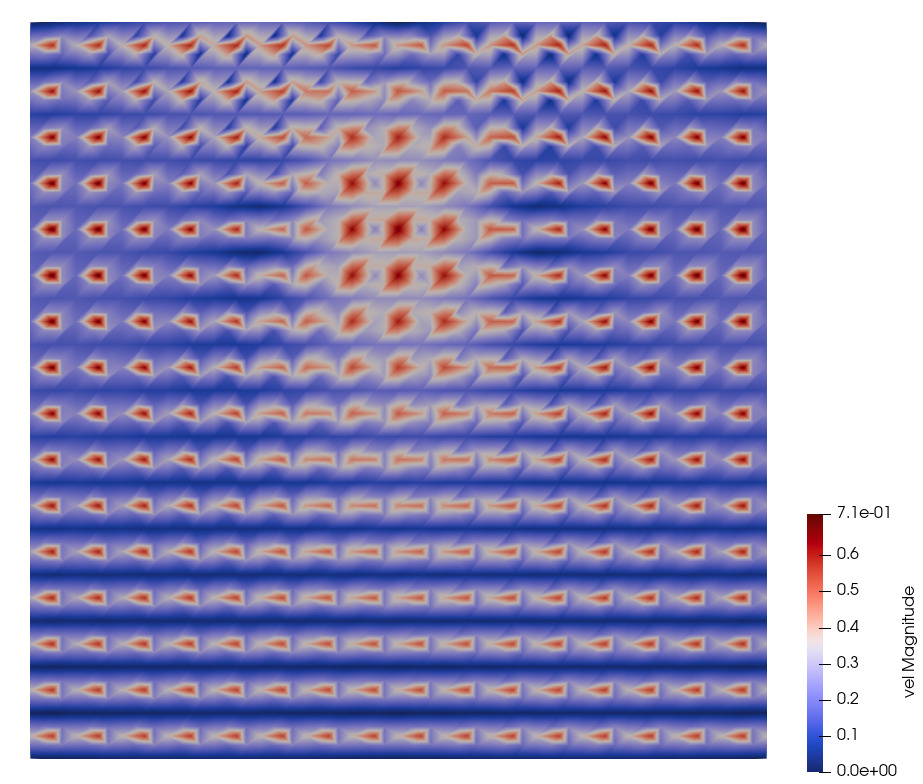
\includegraphics[width=10cm]{python_codes/fieldstone_62/results/vel4}
\end{center}

I believe that one source of our problems when we carried out resolution tests
came from the fact that this small convection cell that occurs as shown above was
always under-resolved. The top layer is 8km thick and the weak zone is 14km thick,
and we ran simulations at max 1km resolution. However, because of the use  
of particle-in-cell and rectangular elements (mostly linear elements), 
a proper capture of this feature in the solution would have required much higher 
resolution. In other words, our higher resolution runs were probably not high resolution enough.
Given the nature of this convection cell, it means that temperature would be advected by it, 
and that markers would likely gotten mixed. 

\newpage
\begin{center}
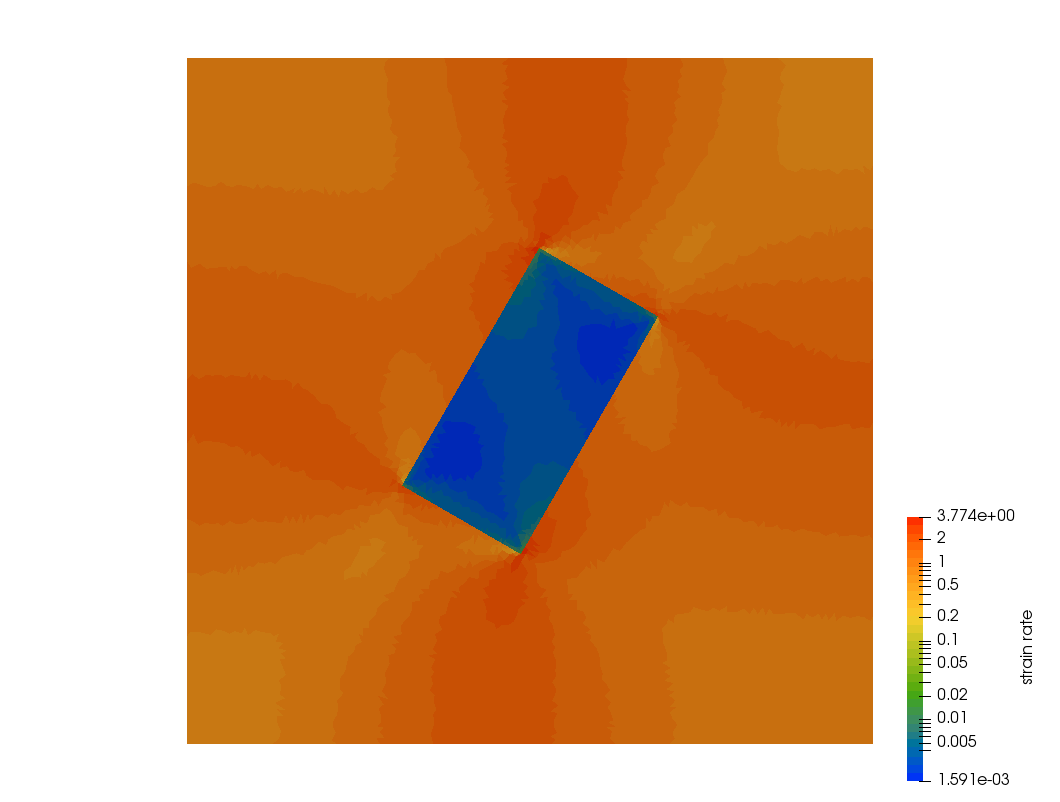
\includegraphics[width=13cm]{python_codes/fieldstone_62/results/sr1}\\
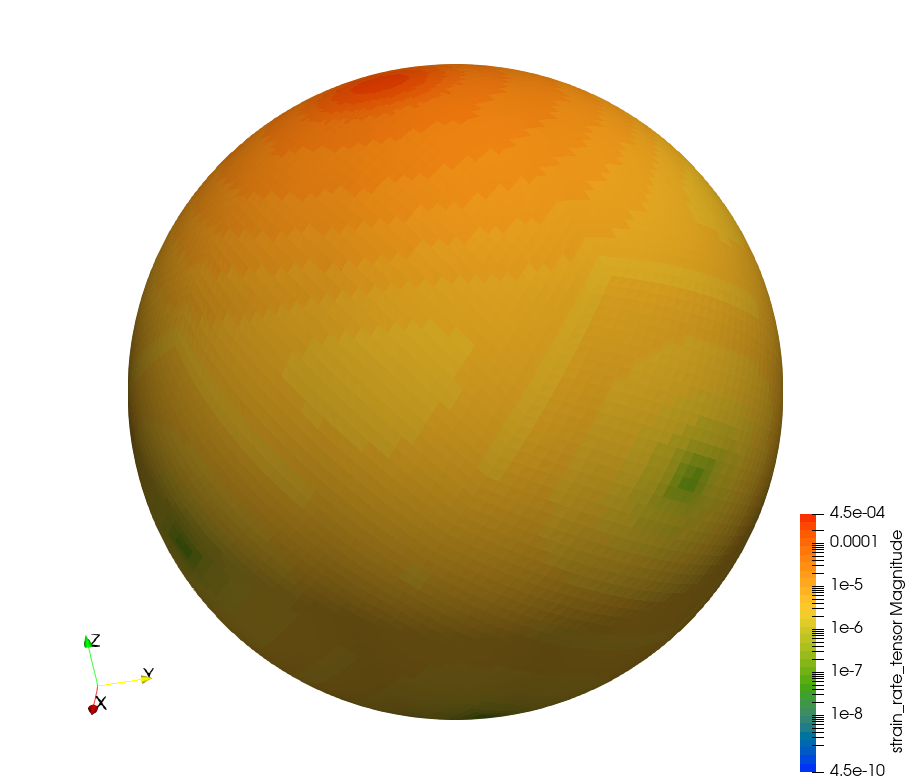
\includegraphics[width=13cm]{python_codes/fieldstone_62/results/sr2}
\end{center}



